\begin{frame}[fragile]{Run Time Polymorphism}
    \begin{columns}[T]
        \begin{column}[T]{5cm}
            \inputminted[mathescape,
                linenos,
                numbersep=5pt,
                frame=lines,
                bgcolor=White,
                fontsize=\tiny,
                linenos,
                framesep=2mm]{c++}
                {/Users/lalanne/MyCode/GitHubProjects/MetaTalk/src/code/run_complex_pol_mine_1.cpp} 
        \end{column}

        \begin{column}[T]{5cm}    
            \inputminted[mathescape,
                       linenos,
                       numbersep=5pt,
                       frame=lines,
                       bgcolor=White,
                       fontsize=\tiny,
                       linenos,
                       framesep=2mm]{c++}
                       {/Users/lalanne/MyCode/GitHubProjects/MetaTalk/src/code/run_complex_pol_mine_2.cpp} 
        \end{column}
    \end{columns}
\end{frame}

\begin{frame}{Run Time Polymorphism}
    \begin{center}
        \begin{tikzpicture}[]
            \node[] at (0mm,0mm){
                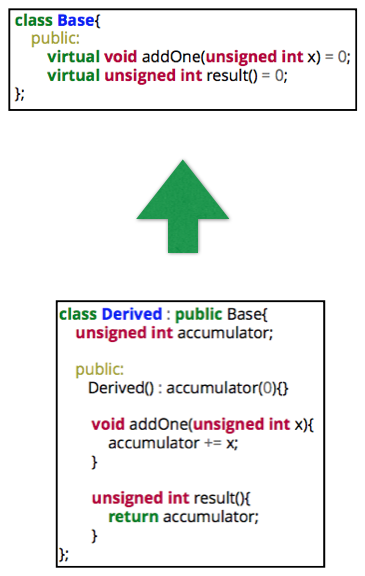
\includegraphics[height=60mm]{/Users/lalanne/MyCode/GitHubProjects/MetaTalk/figures/runcrtpclass.png}\hspace{5mm}
            };
        \end{tikzpicture}
    \end{center}
\end{frame}

\begin{frame}{Run Time Polymorphism}
    \begin{center}
        \begin{tikzpicture}[]
            \node[] at (0mm,0mm){
                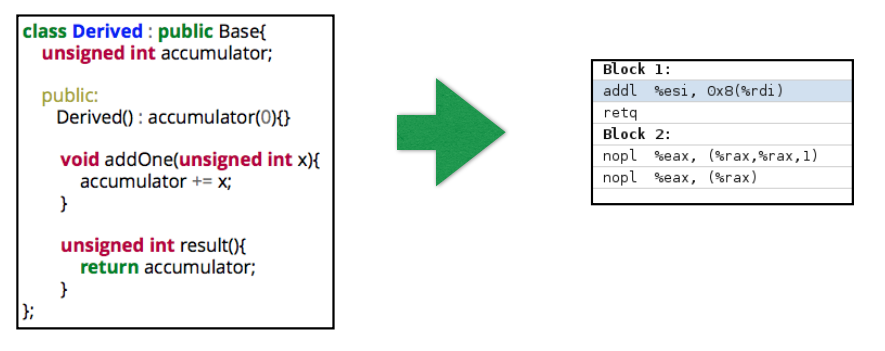
\includegraphics[height=40mm]{/Users/lalanne/MyCode/GitHubProjects/MetaTalk/figures/run_addOne.png}\hspace{5mm}
            };
        \end{tikzpicture}
    \end{center}
\end{frame}

\begin{frame}{Run Time Polymorphism}
    \begin{center}
        \begin{tikzpicture}[]
            \node[] at (0mm,0mm){
                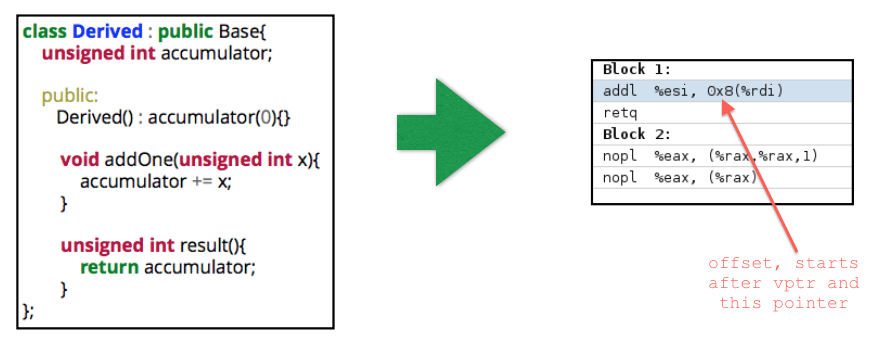
\includegraphics[height=40mm]{/Users/lalanne/MyCode/GitHubProjects/MetaTalk/figures/run_addOne1.png}\hspace{5mm}
            };
        \end{tikzpicture}
    \end{center}
\end{frame}


\begin{frame}{Run Time Polymorphism}
    \begin{center}
        \begin{tikzpicture}[]
            \node[] at (0mm,0mm){
                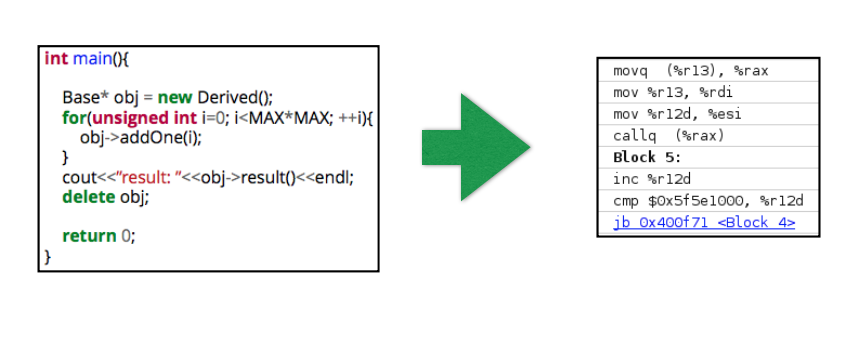
\includegraphics[height=40mm]{/Users/lalanne/MyCode/GitHubProjects/MetaTalk/figures/run_loop_asm.png}\hspace{5mm}
            };
        \end{tikzpicture}
    \end{center}
\end{frame}

\begin{frame}{Run Time Polymorphism}
    \begin{center}
        \begin{tikzpicture}[]
            \node[] at (0mm,0mm){
                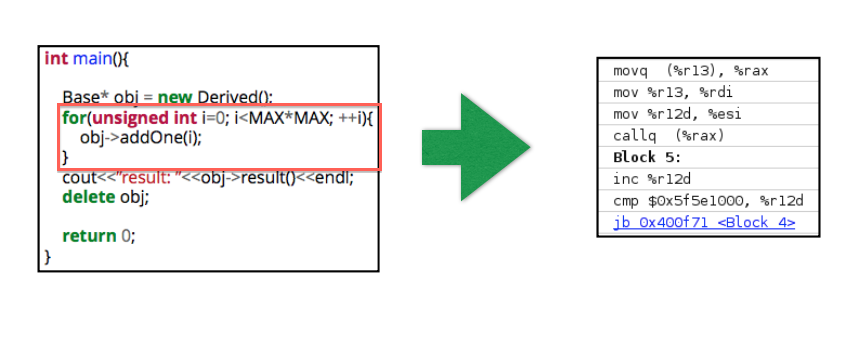
\includegraphics[height=40mm]{/Users/lalanne/MyCode/GitHubProjects/MetaTalk/figures/run_loop_asm1.png}\hspace{5mm}
            };
        \end{tikzpicture}
    \end{center}
\end{frame}

\begin{frame}{Run Time Polymorphism}
    \begin{center}
        \begin{tikzpicture}[]
            \node[] at (0mm,0mm){
                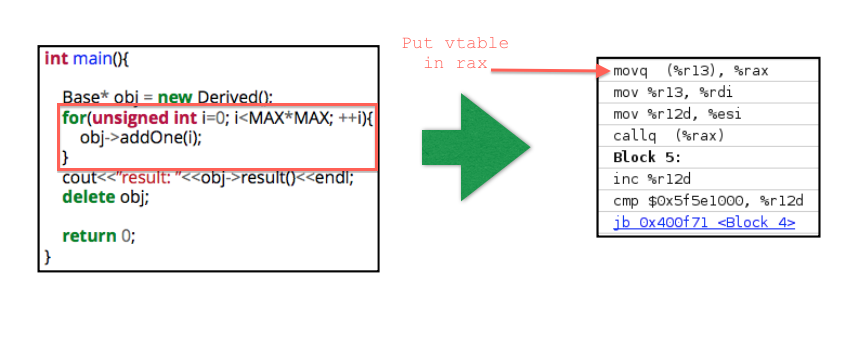
\includegraphics[height=40mm]{/Users/lalanne/MyCode/GitHubProjects/MetaTalk/figures/run_loop_asm2.png}\hspace{5mm}
            };
        \end{tikzpicture}
    \end{center}
\end{frame}

\begin{frame}{Run Time Polymorphism}
    \begin{center}
        \begin{tikzpicture}[]
            \node[] at (0mm,0mm){
                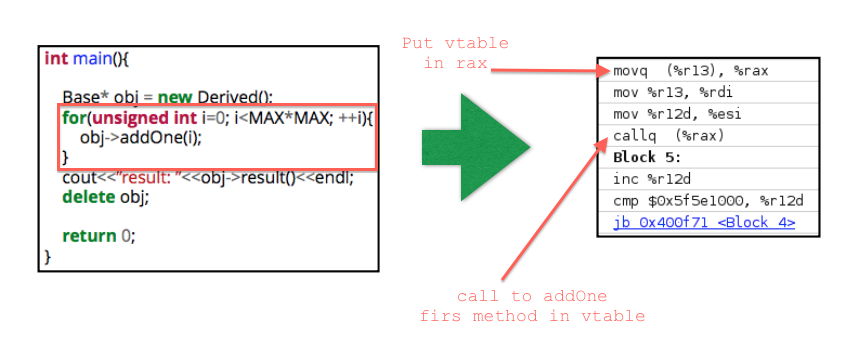
\includegraphics[height=40mm]{/Users/lalanne/MyCode/GitHubProjects/MetaTalk/figures/run_loop_asm3.png}\hspace{5mm}
            };
        \end{tikzpicture}
    \end{center}
\end{frame}

\begin{frame}{Run Time Polymorphism}
    \begin{center}
        \begin{tikzpicture}[]
            \node[] at (0mm,0mm){
                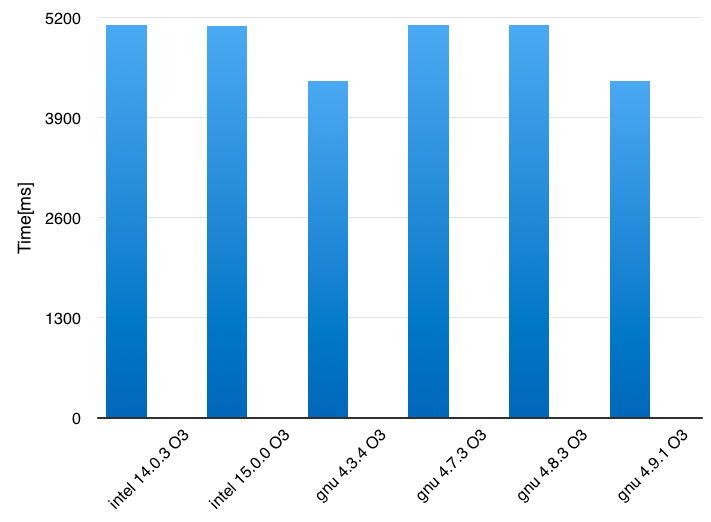
\includegraphics[height=60mm]{/Users/lalanne/MyCode/GitHubProjects/MetaTalk/figures/benchRUN.png}\hspace{5mm}
            };
        \end{tikzpicture}
    \end{center}
\end{frame}

\begin{frame}{Run Time Polymorphism}
    \begin{center}
        \begin{tikzpicture}[]
            \node[] at (0mm,0mm){
                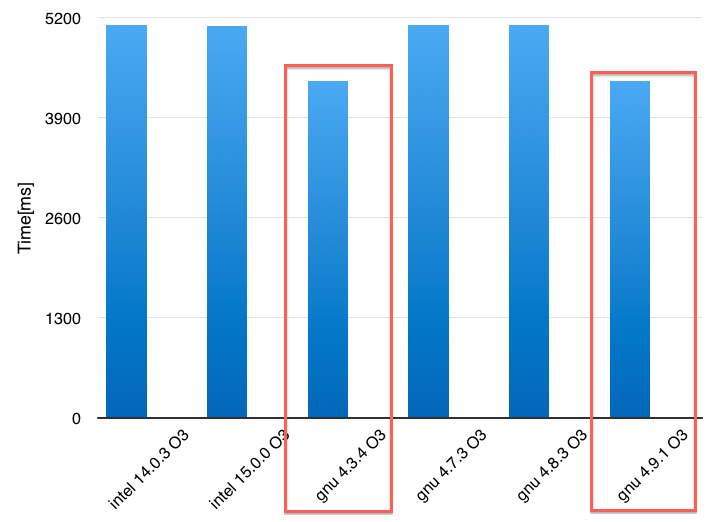
\includegraphics[height=60mm]{/Users/lalanne/MyCode/GitHubProjects/MetaTalk/figures/benchRUN1.png}\hspace{5mm}
            };
        \end{tikzpicture}
    \end{center}
\end{frame}

\begin{frame}[Generate]{Erasing virtual methods, CRTP} 
    \begin{itemize}
        \item Curiously Recurring Template Pattern\cite{eli}.
    \end{itemize}
\end{frame}

\begin{frame}[fragile]{Compile Time Polymorphism}
    \begin{columns}[T]
        \begin{column}[T]{5cm}
            \inputminted[mathescape,
                       linenos,
                       numbersep=5pt,
                       frame=lines,
                       bgcolor=White,
                       fontsize=\tiny,
                       linenos,
                       framesep=2mm]{c++}
                       {/Users/lalanne/MyCode/GitHubProjects/MetaTalk/src/code/comp_complex_pol_mine_1.cpp} 
        \end{column}
        \begin{column}[T]{5cm}
            \inputminted[mathescape,
                   linenos,
                   numbersep=5pt,
                   frame=lines,
                   bgcolor=White,
                   fontsize=\tiny,
                   linenos,
                   framesep=2mm]{c++}
                   {/Users/lalanne/MyCode/GitHubProjects/MetaTalk/src/code/comp_complex_pol_mine_2.cpp}

            \inputminted[mathescape,
                       linenos,
                       numbersep=5pt,
                       frame=lines,
                       bgcolor=White,
                       fontsize=\tiny,
                       linenos,
                       framesep=2mm]{c++}
                       {/Users/lalanne/MyCode/GitHubProjects/MetaTalk/src/code/comp_complex_pol_mine_3.cpp} 
        \end{column}
    \end{columns}
\end{frame}


\begin{frame}{Compile Time Polymorphism}
    \begin{center}
        \begin{tikzpicture}[]
            \node[] at (0mm,0mm){
                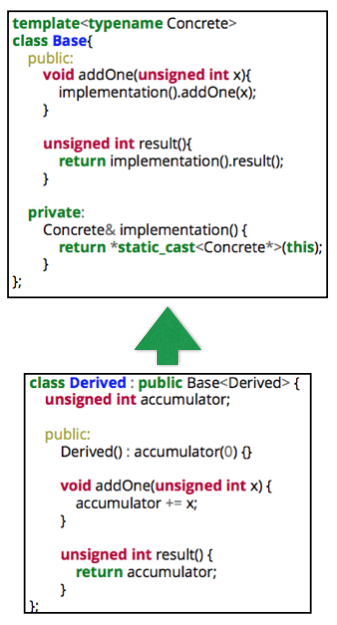
\includegraphics[height=70mm]{/Users/lalanne/MyCode/GitHubProjects/MetaTalk/figures/comp_class.png}\hspace{5mm}
            };
        \end{tikzpicture}
    \end{center}
\end{frame}

\begin{frame}{Compile Time Polymorphism}
    \begin{center}
        \begin{tikzpicture}[]
            \node[] at (0mm,0mm){
                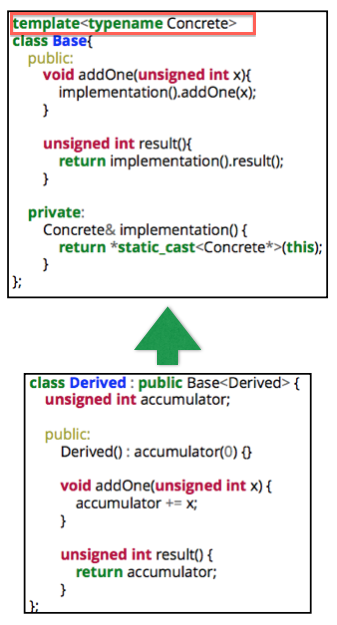
\includegraphics[height=70mm]{/Users/lalanne/MyCode/GitHubProjects/MetaTalk/figures/comp_class1.png}\hspace{5mm}
            };
        \end{tikzpicture}
    \end{center}
\end{frame}

\begin{frame}{Compile Time Polymorphism}
    \begin{center}
        \begin{tikzpicture}[]
            \node[] at (0mm,0mm){
                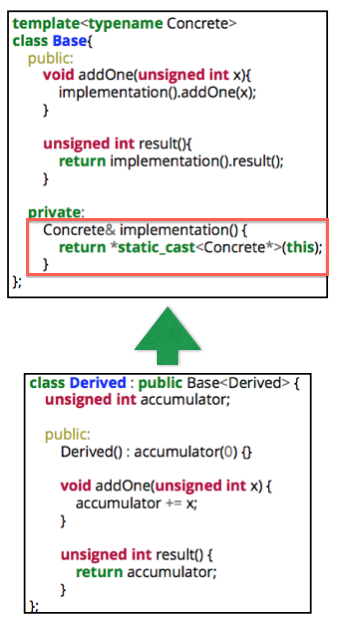
\includegraphics[height=70mm]{/Users/lalanne/MyCode/GitHubProjects/MetaTalk/figures/comp_class2.png}\hspace{5mm}
            };
        \end{tikzpicture}
    \end{center}
\end{frame}

\begin{frame}{Compile Time Polymorphism}
    \begin{center}
        \begin{tikzpicture}[]
            \node[] at (0mm,0mm){
                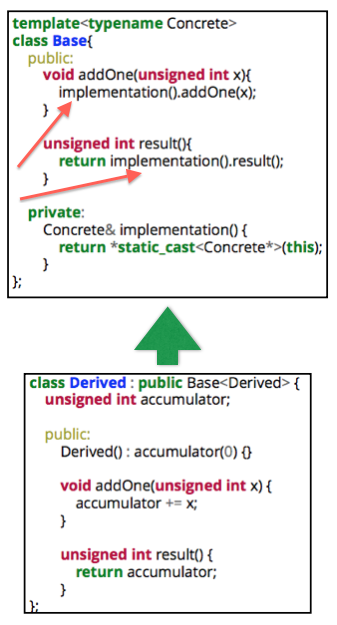
\includegraphics[height=70mm]{/Users/lalanne/MyCode/GitHubProjects/MetaTalk/figures/comp_class2_5.png}\hspace{5mm}
            };
        \end{tikzpicture}
    \end{center}
\end{frame}

\begin{frame}{Compile Time Polymorphism}
    \begin{center}
        \begin{tikzpicture}[]
            \node[] at (0mm,0mm){
                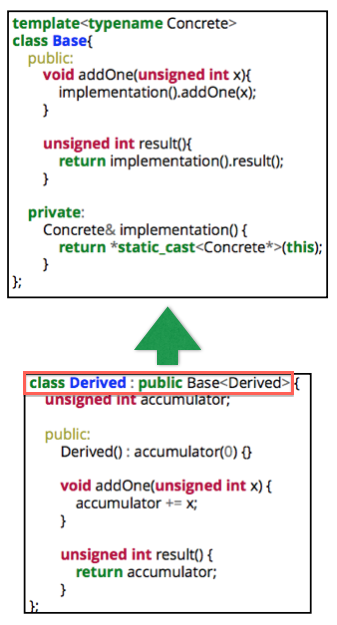
\includegraphics[height=70mm]{/Users/lalanne/MyCode/GitHubProjects/MetaTalk/figures/comp_class3.png}\hspace{5mm}
            };
        \end{tikzpicture}
    \end{center}
\end{frame}

\begin{frame}{Compile Time Polymorphism}
    \begin{center}
        \begin{tikzpicture}[]
            \node[] at (0mm,0mm){
                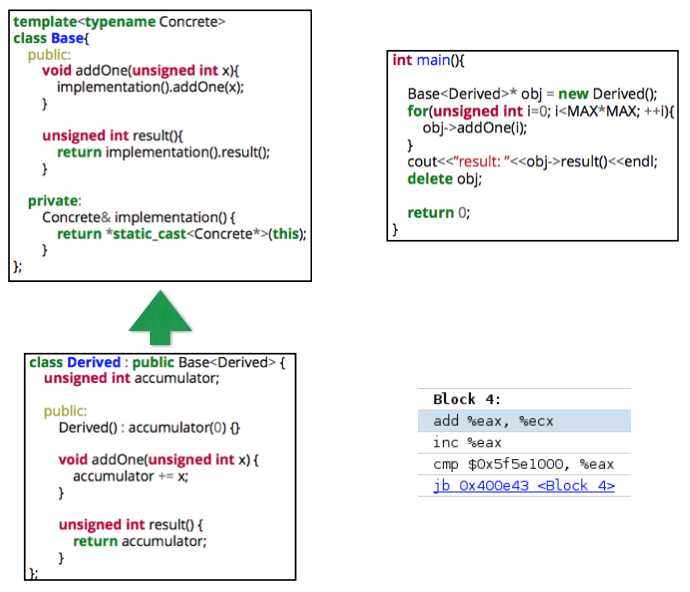
\includegraphics[height=70mm]{/Users/lalanne/MyCode/GitHubProjects/MetaTalk/figures/comp_asm.png}\hspace{5mm}
            };
        \end{tikzpicture}
    \end{center}
\end{frame}

\begin{frame}{Compile Time Polymorphism}
    \begin{center}
        \begin{tikzpicture}[]
            \node[] at (0mm,0mm){
                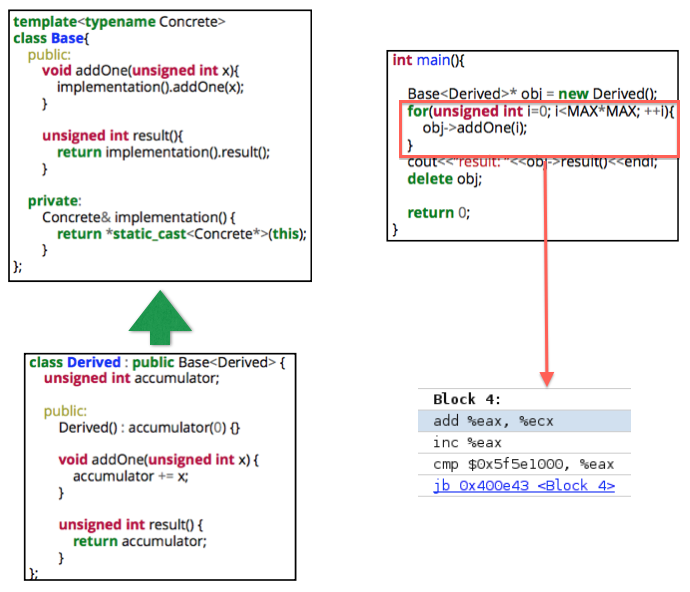
\includegraphics[height=70mm]{/Users/lalanne/MyCode/GitHubProjects/MetaTalk/figures/comp_asm1.png}\hspace{5mm}
            };
        \end{tikzpicture}
    \end{center}
\end{frame}

\begin{frame}{Compile Time Polymorphism}
    \begin{center}
        \begin{tikzpicture}[]
            \node[] at (0mm,0mm){
                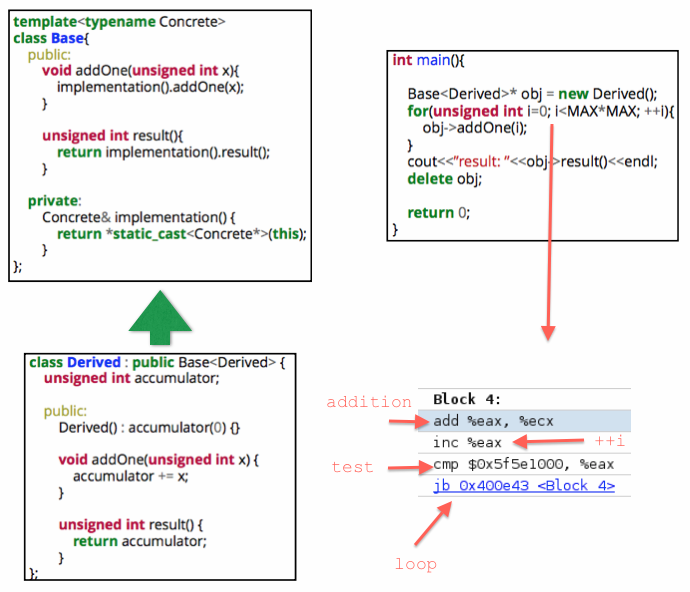
\includegraphics[height=70mm]{/Users/lalanne/MyCode/GitHubProjects/MetaTalk/figures/comp_asm2.png}\hspace{5mm}
            };
        \end{tikzpicture}
    \end{center}
\end{frame}

\begin{frame}{Compile Time Polymorphism}
    \begin{center}
        \begin{tikzpicture}[]
            \node[] at (0mm,0mm){
                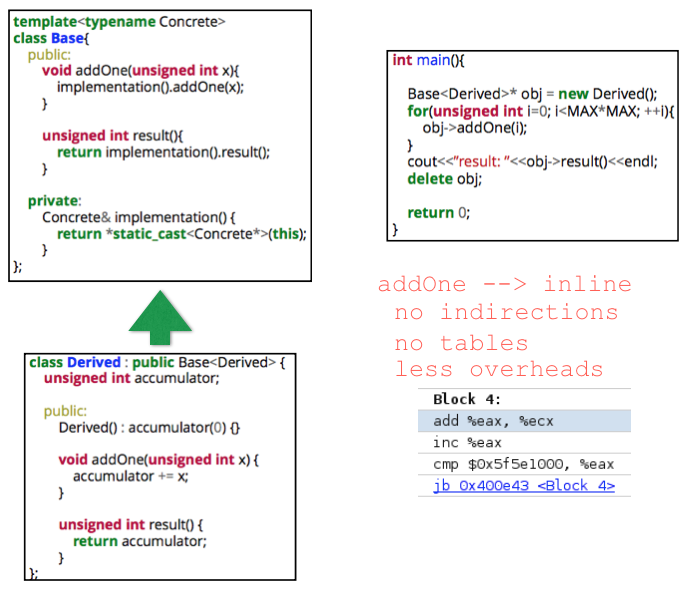
\includegraphics[height=70mm]{/Users/lalanne/MyCode/GitHubProjects/MetaTalk/figures/comp_asm3.png}\hspace{5mm}
            };
        \end{tikzpicture}
    \end{center}
\end{frame}

\begin{frame}{Run Time vs Compile Time}
    \begin{center}
        \begin{tikzpicture}[]
            \node[] at (0mm,0mm){
                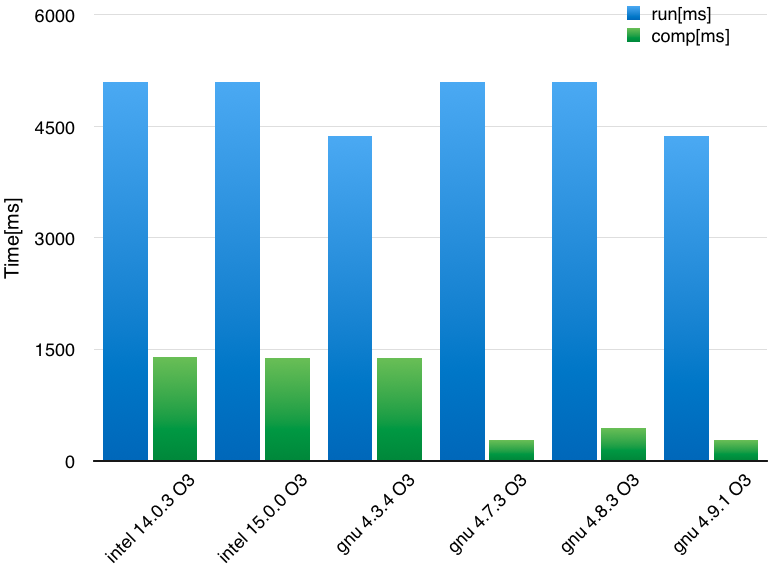
\includegraphics[height=60mm]{/Users/lalanne/MyCode/GitHubProjects/MetaTalk/figures/bench.png}\hspace{5mm}
            };
        \end{tikzpicture}
    \end{center}
\end{frame}

\begin{frame}{Run Time vs Compile Time}
    \begin{center}
        \begin{tikzpicture}[]
            \node[] at (0mm,0mm){
                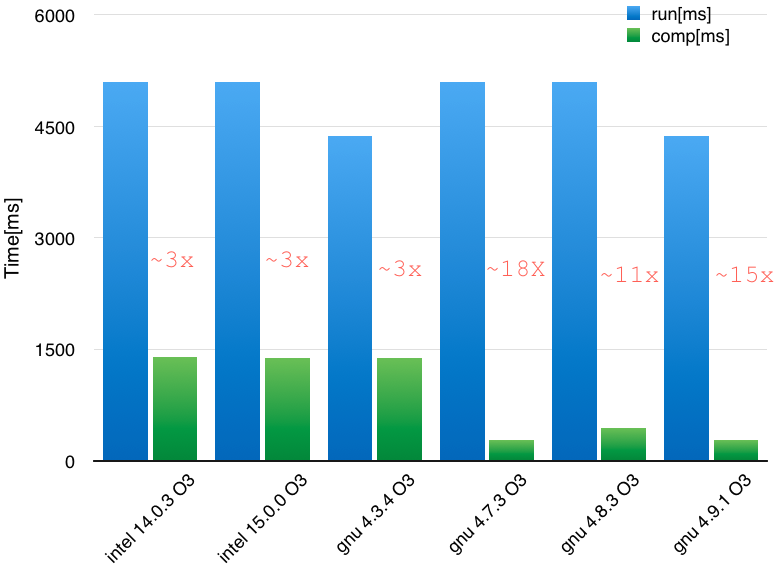
\includegraphics[height=60mm]{/Users/lalanne/MyCode/GitHubProjects/MetaTalk/figures/bench1.png}\hspace{5mm}
            };
        \end{tikzpicture}
    \end{center}
\end{frame}

